\begin{refsection}
%-------------------------------------------------------------------------
%-------------------------------------------------------------------------
\chapter{Optical imperfections in refractive lenses}\label{sec:optical_imperfections}
%-------------------------------------------------------------------------
%-------------------------------------------------------------------------

To understand the impact of CRL on the optical design of complete beamlines, it is necessary to be able to simulate them realistically. The basic implementation of X-ray lenses is already available on the two most widespread beamline simulation tools: \textit{SHADOW} [\cite{SanchezdelRio2011}] and \textit{SRW} [\cite{Chubar1998}]. Both implementations, although based on different schemes, ray tracing [\cite{Alianelli2007}] and wave optics [\cite{Baltser2011}] respectively, are based on an ideal model combining refraction and absorption for the stacked lenses. Much has been done in terms of refining the modelling of ideal X-ray lenses [\cite{Umbach2008, SanchezdelRio2012, Osterhoff2013, Simons2017, Pedersen2018}] and, to a certain extent, the modelling of optical imperfections [\cite{Pantell2001, Andrejczuk2010, Gasilov2017, Osterhoff2017}]. Except for the work presented in [\cite{Roth2014}], investigating and simulating the inner structure of X-ray lenses, the present models consider mainly the lens shape and departure from a perfect parabolic shape. The majority of these models, however, is not publicly available, nor are readily compatible with standard beamline simulations suits like \textit{SHADOW} and \textit{SRW}. Another bottle-neck to the current literature or computer codes for simulating CRLs is that they do not include the data from real lenses metrology, as is routinely done for X-ray mirrors simulations [\cite{SanchezDelRio2016}], which undermines the inclusion of CRLs in simulations of complete beamline configurations in combination with other optical elements.

The modelling and functions presented here\footnote{This first section in this chapter, \S\ref{sec:describing_modelling}~-~\textit{\nameref{sec:describing_modelling}}, is partially based on the work originally published in [\cite{Celestre2020b}].} are based on the framework of physical optics (cf. \S\ref{sec:physical_optics}~-~\textit{\nameref{sec:physical_optics}}) and are tailored to be used transparently with SRW [\cite{Chubar1998}], which already provides a model for the CRL [\cite{Baltser2011}] - this basic ideal model combines refraction and absorption for the stacked lenses; optical imperfections from material inhomogeneities (voids, impurities) were later added [\cite{Roth2014}]. Expanding this model, we present the optical imperfections in refractive lenses in three different groups: \textit{i}-) misalignments of a single X-ray lens; \textit{ii}-) commonly encountered fabrication errors such transverse offsets as well as tilts of the individual parabolic sections; \textit{iii}-) and other sources of deviations from the parabolic shape modelled with either polynomial decomposition of error functions or by using metrology data. Each newly added feature is accompanied by a calculation of the residual thickness error, its impact on focusing by CRL and the beam caustic in the vicinity of the focal spot\footnote{All simulations shown throughout this chapter have similar conditions, that is, they model misalignments, fabrication errors or arbitrary residual errors to a single 2D-Beryllium lens with nominal radius $R=50~\mu\text{m}$, geometric aperture $A_{\diameter}=440~\mu\text{m}$ and $t_\text{wall}=20~\mu$m at 8~keV in fully-coherent simulations. The illumination is filament electron beam passing through a CPMU18 undulator with 111 magnetic periods with $\Lambda=18$~mm magnetic period and magnetic field $B=0.9863~$T - cf. \S\ref{sec:brilliance}~-~\textit{\nameref{sec:brilliance}}. The electron-beam parameters are the ones from the ESRF-EBS upgrade [\cite{orangebook}]. An ideal parabolic phase element with radius of curvature $R=-60~$m is placed 60~m downstream the radiation source to give the illumination a near-plane phase - cf. Eq.~\ref{eq:planewave}, so that the PSF and beam caustics can be calculated. The application of the presented modelling to partially-coherent simulations methods [\cite{Chubar2011}] is shown in \S\ref{sec:effect_optical_imperfections}~-~\textit{\nameref{sec:effect_optical_imperfections}}.}, which are summarised in Fig.~\ref{fig:Strehl_modelling}. Calculations presented in this chapter are merely illustrative and a systematic evaluation is presented in \S\ref{sec:effect_optical_imperfections}~-~\textit{\nameref{sec:effect_optical_imperfections}}. The code main functions implementing the ideal CRL and describing optical imperfections in refractive lenses are subsequently presented. The metrology technique used to obtain the phase errors that arise from material inhomogeneities (voids, impurities) and/or figure errors from the lens forming process, namely, X-ray speckle tracking, is discussed at length. After considerations on data processing and analysis, a selection of experimental data is discussed and corrective optics based on the metrology data is proposed. 


\begin{figure}[t]
    \centering
    {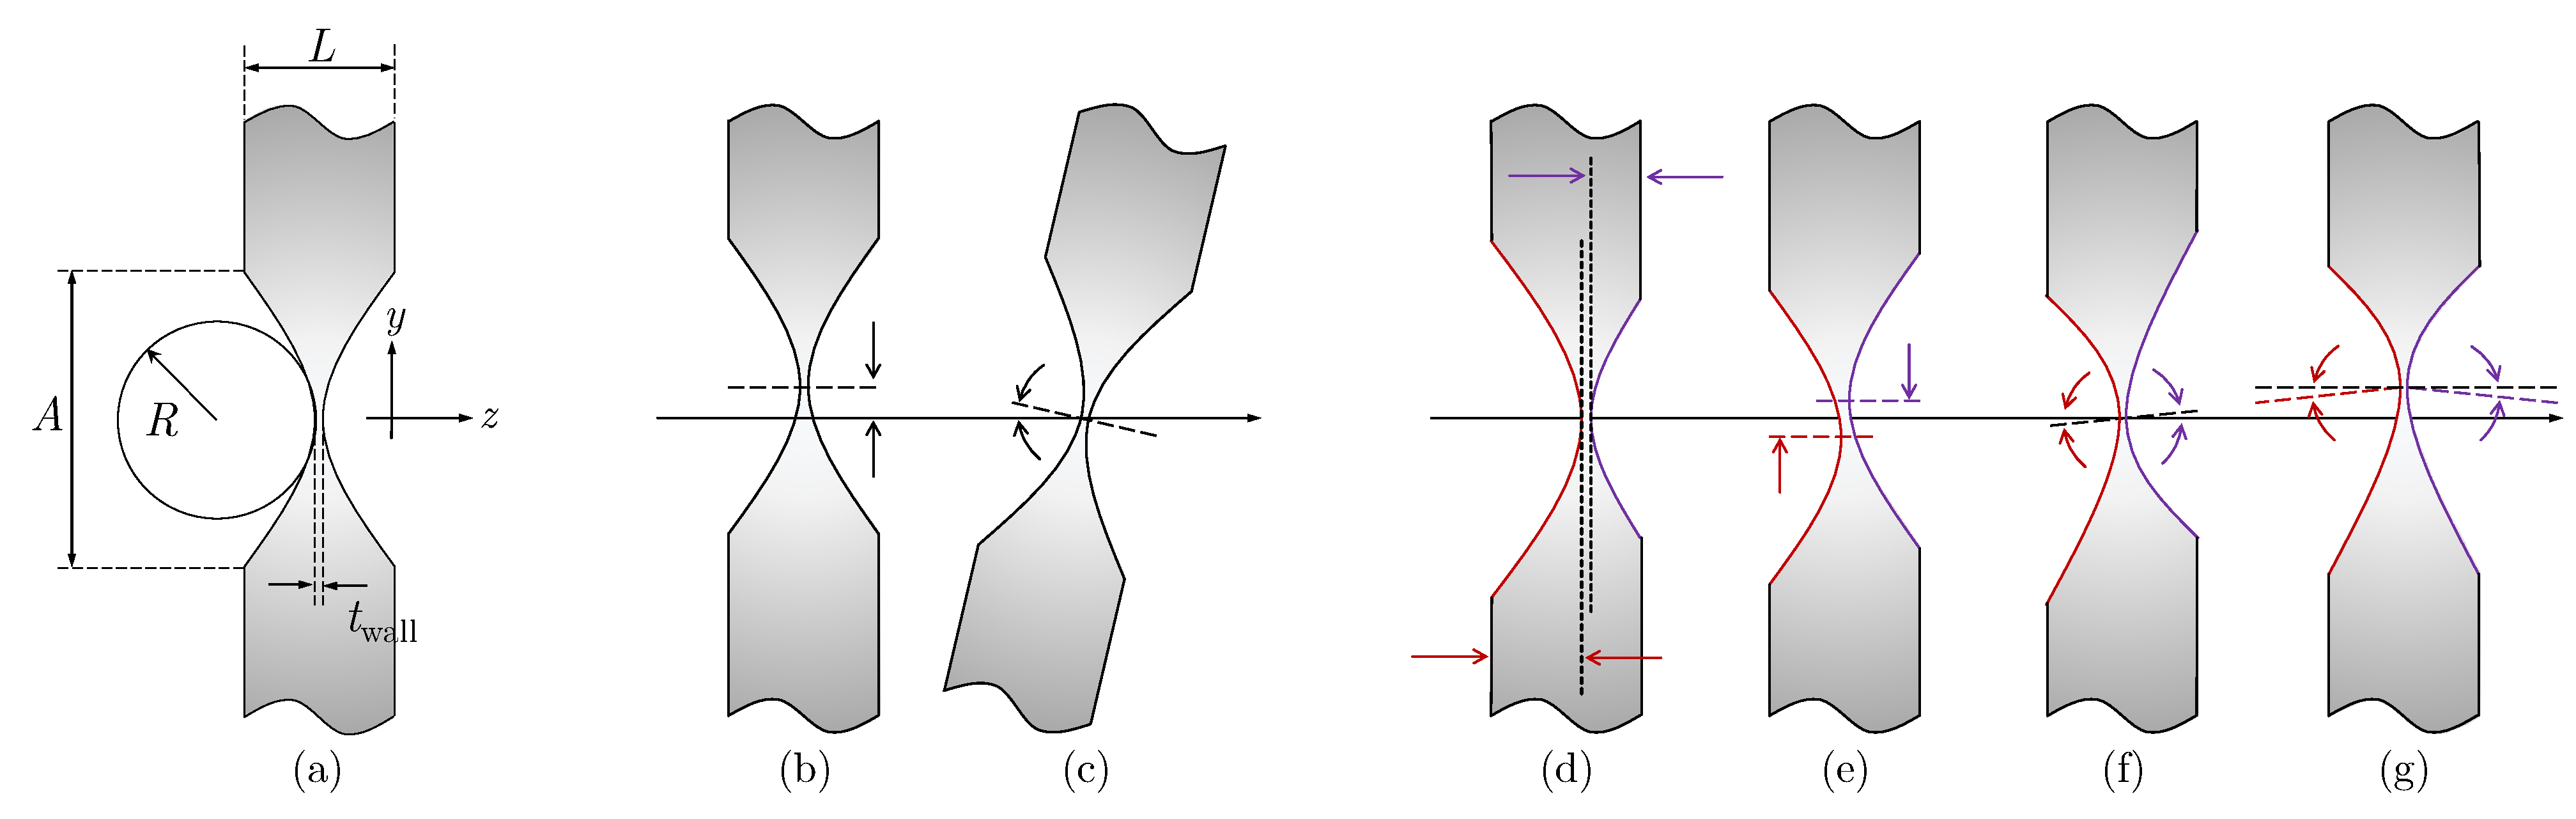
\includegraphics[width=1.\linewidth]{figures/ch04/lens_cuts.pdf}}
    \caption[Modelling misalignments and fabrication errors in CRLs]{(a) ideal lens for reference. Lens typical misalignments are the (b) transverse offset and the (c) tilt or a combination of both. Common fabrication errors include the (d) longitudinal offset of the parabolic section, (e) transverse offset of the parabolic section and (f)-(g) tilted parabolic sections.}
    \label{fig:lens_cuts}
\end{figure}

%-------------------------------------------------------------------------
%-------------------------------------------------------------------------
\section{Describing and modelling optical imperfections in refractive lenses}\label{sec:describing_modelling}
%-------------------------------------------------------------------------
%-------------------------------------------------------------------------

In the paraxial approximation, the parabolic shape for a refracting surface is generally regarded as the ideal shape\footnote{The shape of a focusing refracting surface can be derived from the Fermat's principle, but the parabolic shape is generally regarded as a good approximation. Large apertures are often necessary when very small focused beams are required, but increasing the geometric aperture of the optical element causes the parabolic approximation to under-perform. Several aspheric surface shapes for different focusing conditions were reported in [\cite{SanchezdelRio2012}] - cf. Fig~4. For a deeper discussion on aspheric surfaces in the context of optics, please, refer to [\cite{Schulz1988}].} for minimising aberrations. It is legit, then, to define as errors any deviation from this ideal parabolic form\footnote{Such definition, however, leaves out discrepancies in the radius of curvature $R$ (designed vs. \textit{de facto}) and the associated defocus it may cause. Discrepancies between designed and executed lenses may render them to be labelled as out-of-specification and may cause the system to under-perform, but are not deviations of the parabolic shape, provided the ideal parabolic shape takes into account the \textit{de facto} radius of curvature. Accounting for such discrepancies can be done using the ideal model described by the transmission element $\mathrm{T}_{\text{single lens}}(\Delta_z)$ (cf. Eq.~\ref{eq:TE_singlelens}) using the \textit{de facto} radius of curvature.} regardless of its origin. The phase errors induced by an ideal lens misalignment will be presented first, then the typical fabrication errors of bi-concave lenses will be presented shortly after. The misalignment and fabrications errors presented in this section were derived from the accumulated experience in handling beryllium and aluminium bi-concave embossed lenses, which are the most available throughout beamlines in diverse synchrotron facilities. However, the modelling presented here is generic and can be applied to a wide-range of CRL from diverse fabrication processes\footnote{cf. Table~1 from the supplementary material relative to [\cite{Roth2017}].}. Fig.~\ref{fig:ideal_CRL} shows the focusing performance of a single ideal 2D-Beryllium lens with nominal radius $R=50~\mu\text{m}$, geometric aperture $A_{\diameter}=440~\mu\text{m}$ and $t_\text{wall}=20~\mu$m at 8~keV using the SRW basic modelling. 
 \begin{figure}[t]
        \centering
        {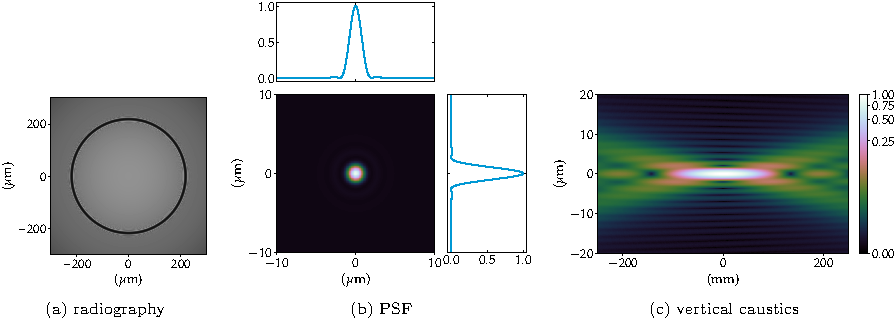
\includegraphics[height=4.19cm]{figures/ch04/CRL_ideal.pdf}}
        \caption[The ideal single X-ray lens]{Simulations of a single ideal 2D-Beryllium lens with nominal radius $R=50~\mu\text{m}$, geometric aperture $A_{\diameter}=440~\mu\text{m}$ and $t_\text{wall}=20~\mu$m at $8$~keV  - cf. Fig~\ref{fig:lens_cuts}(a). (a) phase-contrast image $150~$mm downstream the ideal lens, (b) point-spread function with cuts centred in $(0,0)$ and (c) the vertical beam caustics from $-250$~mm to $250$~mm in respect to the focal plane at $f=4.700~$m.} \label{fig:ideal_CRL}
\end{figure}


%-------------------------------------------------------------------------
%-------------------------------------------------------------------------
\subsection{Misalignments}\label{sec:misalignments}
%-------------------------------------------------------------------------
%-------------------------------------------------------------------------

Misalignments of optical systems are not optical errors \textit{per se} as they can be mitigated by ensuring proper alignment is done; they will, however, cause changes to the ideal parabolic phase profile if left uncorrected and will affect the optical performance of the system. Although aligning a CRL stack is possible\footnote{The possibility of realignment of the CRL depends on where and how they are installed in the beamline. If their installation is on a bulky transfocator [\cite{Vaughan2011}], their realignment is more difficult to be performed. However, when used as a final focusing element, enclosed in small casings or compact transfocators - cf. Fig.~3 in [\cite{Lengeler1999}] and [\cite{Kornemann2017, Narikovich2019}], their realignment can be done more easily.}, the individual lenslets usually cannot be aligned to each other, hence the interest in modelling such misalignments.

%-------------------------------------------------------------------------
%-------------------------------------------------------------------------
\subsubsection*{Transverse offset}
%-------------------------------------------------------------------------
%-------------------------------------------------------------------------

Shifting transversely a single element an transverse distance $(\Delta_x,\Delta_y)$ can be simply done by calculating $\Delta_z(x-\Delta_x,y-\Delta_y)$ in Eq.~\ref{eq:ProjecThick}. The shifted element is depicted in Fig.~\ref{fig:lens_cuts}(b). For a pair of coordinates $(x,y)$:
\begin{equation}\label{eq:ProjecThick_misaligned}
    \Delta_z(x-\Delta_x,y-\Delta_y) = 
        \begin{cases}
      \cfrac{(x-\Delta_x)^2}{R_x}+\cfrac{(y-\Delta_y)^2}{R_y}+\text{t}_\text{wall}, &\quad\forall~(x-\Delta_x,y-\Delta_y) \in A,\\
      L, &\quad\text{otherwise}.
        \end{cases}
\end{equation}   
Eq.~\ref{eq:ProjecThick_misaligned} is the ideal parabolic profile of a bi-concave lens given by Eq.~\ref{eq:ProjecThick} with its vertices centred around $(\Delta_x,\Delta_y)$. While a single transversely shifted lens considered on its own is innocuous, piling up several shifted lenses has impacts on the overall accumulated phase parabolic shape and resulting geometric aperture. Although the exact effect of relative misaligments between individual lenses on the phase of the wave-field depends on the distance between lenslets, the energy, footprint and divergence of the X-ray beam, some insight can be gained by considering the individual focusing elements as thin-optical elements in intimate contact. Consider $N$ stacked lenses transversely misaligned with their transverse distance to the optical axis given by $(\Delta_{x_j},\Delta_{y_j})$, with $j=1,~2,~...,~N$. Within the intersection of their geometric apertures, the accumulated thickness is given by:
% \begin{subequations}
\begin{align}\label{eq:ProjecThick_Nmisaligned}
    \Delta_{z_\Sigma}(x,y) &= \sum\limits_{j=1}^N \Delta_z(\Delta_{x_j},\Delta_{y_j})\nonumber\\
    &=\sum\limits_{j=1}^N \underbrace{\frac{x^2}{R_{x_j}}+\frac{y^2}{R_{y_j}}}_\text{(I)}
    -\underbrace{2x\frac{\Delta_{x_j}}{R_{x_j}} - 2y\frac{\Delta_{y_j}}{R_{y_j}}}_\text{(II)}
    +\underbrace{\frac{\Delta_{x_j}^2}{R_{x_j}}+\frac{\Delta_{y_j}^2}{R_{y_j}}+\text{t}_{\text{wall}_j}}_\text{(III)}.
\end{align}
The first term in Eq.~\ref{eq:ProjecThick_Nmisaligned}, ($\text{I}$) is a quadratic term and it indicates ideal focusing as in Eq.~\ref{eq:ProjecThick}. The residual terms ($\text{II}$) and ($\text{III}$) are a linear term in $x$ and $y$ and a constant offset term, respectively. The projected thickness and the phase are linearly proportional, so the residual accumulated thickness translates directly into residual accumulated phase and both terms can be used interchangeably - cf. Eq.\ref{eq:aux_funcs_transb}. The first residual term, i.e. ($\text{II}$), adds a linear phase to the wave-front and acts like a prism, not deforming the monochromatic wave-field, but redirecting it. At the focal plane, the image position is transversely shifted but no change to the intensity and phase profiles is added. Symmetrically shifted lenses\footnote{That is $\Delta_{x_m}=-\Delta_{x_n}$ or $\Delta_{y_m}=-\Delta_{y_n}$ for $m,n\in(1,~2,~...,~N)$.} make ($\text{II}$) goes to zero. The residual terms in ($\text{III}$) add a constant phase offset to the transmitted beam. The effects of the transverse offset to a single X-ray lens are shown in Fig.~\ref{fig:shifted_CRL}.
\begin{figure}[t]
        \centering
         {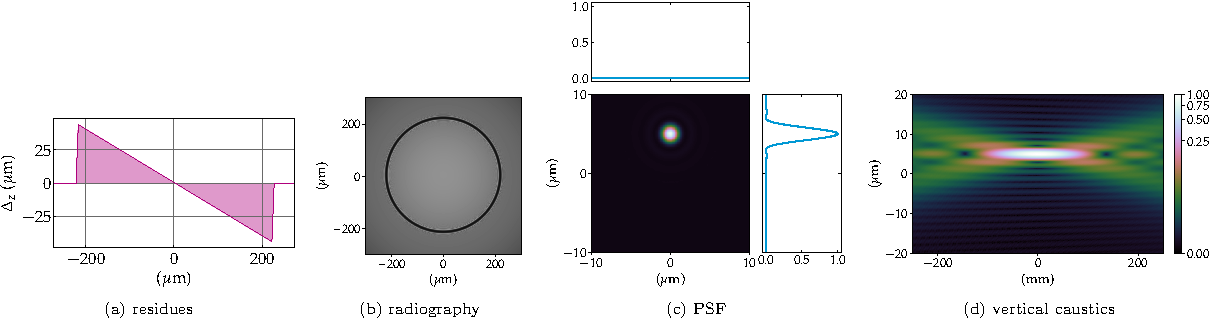
\includegraphics[height=4.19cm]{figures/ch04/shifted_CRL.pdf}}
        \caption[Effects of a transverse CRL offset]{Simulations of an ideal lens shifted by $\Delta_y=5~\mu$m - cf. Fig~\ref{fig:lens_cuts}(b). (a) Residual thickness, (b) phase-contrast image $150~$mm downstream the lens, (c) point spread function with cuts centred in $(0,0)$ and (c) the vertical beam caustics from $-250$~mm to $250$~mm in respect to the focal plane at $f=4.700~$m.} \label{fig:shifted_CRL}
\end{figure}


%-------------------------------------------------------------------------
%-------------------------------------------------------------------------
\subsubsection*{Tilted lens}
%-------------------------------------------------------------------------
%-------------------------------------------------------------------------
\begin{figure}[t]
        \centering
        {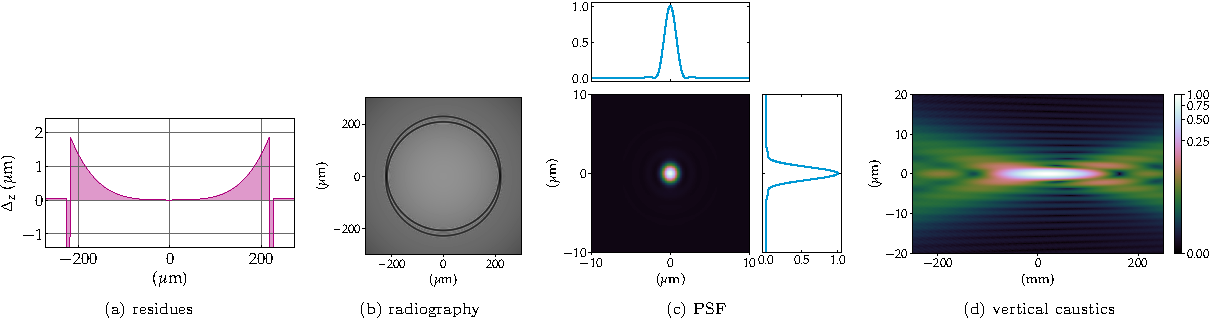
\includegraphics[height=4.19cm]{figures/ch04/tilted_CRL.pdf}}
        \caption[Effects of a CRL tilt]{Simulations of an ideal lens tilted by $\theta_x=1^{\circ}$ - cf. Fig~\ref{fig:lens_cuts}(c). (a) Residual thickness, (b) phase-contrast image $150~$mm downstream the lens, (c) point spread function with cuts centred in $(0,0)$ and (c) the vertical beam caustics from $-250$~mm to $250$~mm in respect to the focal plane at $f=4.700~$m. The profile shown in (a) is proportional to the 4$^{\text{th}}$ power of the lateral coordinates in the direction of the shift. This contributes for the elongation of the beam along the propagation direction and shift on the focal plane position as evidenced by (d), which is a typical sign of spherical aberrations.} \label{fig:tilted_CRL}
\end{figure}

When rotating a lens in space as shown in Fig.~\ref{fig:lens_cuts}(c) and calculating its projected thickness, it is helpful to decouple the rotation of the front and back surfaces. This can be done by defining a point cloud in Cartesian coordinates:
\begin{subequations}\label{eq:point_cloud}
    \begin{align}
    z_\text{front surface}(x-\Delta_x,y-\Delta_y) &=\frac{\Delta_z(x-\Delta_x,y-\Delta_y)}{2},\\
    z_\text{back surface}(x-\Delta_x,y-\Delta_y) &= -\frac{\Delta_z(x-\Delta_x,y-\Delta_y)}{2}
    \end{align}
\end{subequations}{}
where $\Delta_z(x-\Delta_x,y-\Delta_y)$ is given by Eq.~\ref{eq:ProjecThick_misaligned}. The projected thickness is given by:
\begin{align}\label{eq:point_cloud_thickness}
    \Delta_z(x,y) = z_\text{front surface}(x,y) - z_\text{back surface}(x,y),
\end{align}{}
provided those are calculated on the same grid $(x,y)$. A tilted lens can be described by rotation matrices in three dimensions. The transformation matrices allowing a rotation $\theta_{x,y,z}$ around each of the Cartesian axis are~[\cite{House2016}]:
\begin{subequations}\label{eq:affine}
    \begin{align}
        R_x &= \begin{bmatrix}
                            1 & 0 & 0 &0\\
                            0 & \cos\theta_x & -\sin{\theta_x}  &0\\
                            0 & \sin\theta_x & \cos\theta_x &0\\
                            0 & 0 & 0 &1
            \end{bmatrix}  &&(\small{\text{rotation around the $x-$axis}}),\\
            R_y &= \begin{bmatrix}
                            \cos\theta_y & 0 & \sin\theta_y &0\\
                            0 & 1 & 0 &0\\
                            -\sin\theta_y & 0 & \cos\theta_y &0\\
                            0 & 0 & 0 &1
            \end{bmatrix}  &&(\small{\text{rotation around the $y-$axis}}),\\
            R_z &= \begin{bmatrix}
                            \cos\theta_z & -\sin\theta_z & 0 &0\\
                            \sin\theta_z & \cos\theta_z & 0 &0\\
                            0 & 0 & 1 &0\\
                            0 & 0 & 0 &1
            \end{bmatrix}  &&(\small{\text{rotation around the $z-$axis}}).
    \end{align}
\end{subequations}{}
Matrix multiplication is associative, which implies that if multiple rotations are involved, that is $R_x, R_y$ and $R_z$ are applied to a set of points $(x,y,z)$, an equivalent rotation matrix $R_{\theta}=R_zR_yR_x$ can be calculated and then, applied to those points is space: 
\begin{align}\label{eq:affine2}
    [x_\theta,y_\theta,z_\theta,1]^\text{T} & = R_zR_yR_x[x,y,z,1]^\text{T},\nonumber \\
     & = R_\theta[x,y,z,1]^\text{T},
\end{align}{}
where $(x_\theta,y_\theta,z_\theta)$ are the transformed $(x,y,z)$ coordinates after the $R_{\theta}=R_zR_yR_x$ rotation and the $^\text{T}$ in Eq.~\ref{eq:affine2} represents transposed matrices. The rotations given by $R_{\theta}$ have to be applied to both the front and back surfaces of the lens independently, with their respective point clouds given by Eqs.~\ref{eq:point_cloud}. In order to calculate the projected thickness along the optical axis, the rotated front and back surfaces have to be recalculated on a common grid, which is done by two-dimensional interpolation of $(x_\theta,y_\theta,z_\theta)$ to the original $(x,y)$ grid. The associative property allows for considerable computation time reduction, as the rotation can be done applying a single equivalent rotation matrix as opposed to three individual rotations. On the other hand, matrix multiplication is not commutative and the order of operations matter and should be specified\footnote{The implementation of the affine transformations for rotating CRLs in space follow the order: rotation around the $x-$axis ($R_x$), rotation around the $y-$axis ($R_y$) and then, rotation around the $z-$axis ($R_z$).}$^{,}$\footnote{For a deeper discussion on the properties of the affine transformations, coordinates systems and quaternions, please refer to appendices \textit{C}-\textit{E} in [\cite{House2016}].} when rotating a point cloud. Equations~\ref{eq:affine} have their pivot point centred in the origin of their axis, that is, around $(x,y,z)=(0,0,0)$ in Cartesian coordinates. It is possible to define arbitrary pivot points with a combination of translations and rotations. Tilting an optical element in space will introduce aberrations to the beam propagation and its focusing\footnote{The interest in tilted optical elements and compensation is an active field, as evidenced by the literature on that subject - cf. [\cite{Guizar-Sicairos2011,Zhou2019,Ali2020}].}. This is evidenced by the residual accumulated thickness in projection approximation shown in Fig.~\ref{fig:tilted_CRL}. It is also possible to see how the two surfaces (back and front) do not overlap, causing a slight reduction in the geometric aperture area, which is evidenced by the discontinuities in Fig.~\ref{fig:tilted_CRL}(a).

%-------------------------------------------------------------------------
%-------------------------------------------------------------------------
\subsection{Fabrication errors}\label{sec:fabrication}
%-------------------------------------------------------------------------
%-------------------------------------------------------------------------

Modelling the typical misalignment of X-ray lenses implies calculating the lateral displacements and rotations in space of an ideal X-ray lens. However, bi-concave lenses may also present misalignments between the front and back focusing surfaces, these are closely related to the manufacturing processes involved in the lens production. Here, the front and back focusing surfaces are treated independently, allowing to model longitudinal and transverse misalignments as well as tilts of the front and back focusing surface concerning the optical axis.


%-------------------------------------------------------------------------
%-------------------------------------------------------------------------
\subsubsection*{Longitudinal offset of the parabolic section}
%-------------------------------------------------------------------------
%-------------------------------------------------------------------------
Longitudinal offsets of the parabolic portions of a bi-concave X-ray lens appear when, for the same radius of curvature $R$, one parabolic portion is deeper than the other one - cf. Fig.~\ref{fig:lens_cuts}(d). The first eminent observation if that front and back surfaces will have different geometric apertures along the focusing direction. The new geometric aperture of the longitudinally offset parabolic profile can be calculated as:
\begin{equation}\label{eq:A_2}
    A_{\text{offset}} = 2\sqrt{[L-(\text{t}_\text{wall}+2\cdot\text{offset})]R},
\end{equation}{}
where a positive offset increases the apparent web thickness of the half lens to $\text{t}_\text{wall}/2+\text{offset}$ and decreases the geometric aperture for a fixed lens thickness. The aperture given by $ A_{\text{offset}}$ and the apparent web thickness are used in Eq.~\ref{eq:point_cloud_thickness} (cf. Eqs.~\ref{eq:ProjecThick_misaligned} and \ref{eq:point_cloud}) when calculating the projected thickness.
Longitudinal offsets do not affect the parabolic accumulated shape of a single lens and, consequently, do not impose any optical imperfection to an optical system based on such lenses. However, they are often encountered in real lenses\footnote{Specially in embossed lenses, where different penetration depths of the punches often lead to asymmetric lenses.} and merit the implementation in the lens modelling. Fig.~\ref{fig:longitudinal_offset} shows the simulated profile and a radiography of a real lens showing the effects of the longitudinal offset of the parabolic section.

\begin{figure}[t]
        \centering
        {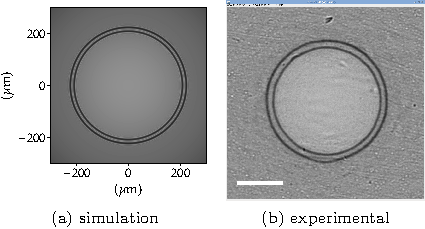
\includegraphics[height=3.cm]{figures/ch04/longitudinal_offset.pdf}}
        \caption[Effects of the longitudinal offset of the parabolic section]{(a) Simulated and (b) measured phase-contrast image of a single of a 2D-Beryllium lens with nominal radius $R=50~\mu\text{m}$ with designed geometric aperture $A_{\diameter}=440~\mu\text{m}$. The scale bar in (b) is worth $200~\mu$m.} \label{fig:longitudinal_offset}
\end{figure}

%-------------------------------------------------------------------------
%-------------------------------------------------------------------------
\subsubsection*{Transverse offset of the parabolic section}
%-------------------------------------------------------------------------
%-------------------------------------------------------------------------

Although parallel to the optical axis, it is possible that the parabolic surfaces axes are not collinear. This is shown in Fig.~\ref{fig:lens_cuts}(e). The modelling of the transverse offset of the front or/and back surfaces of a lens concerning the optical axis is done by calculating the net offset of each surface, that is the sum of lens transverse offset with the front or/and back surface transverse offset, and applying it to Eqs.~\ref{eq:point_cloud} when calculating Eq.~\ref{eq:point_cloud_thickness}. The effects on the residual accumulated phase of non-collinear parabolic surfaces are the same as the one described in the section \textit{Transverse offset} from \S\ref{sec:misalignments}~-~\textit{\nameref{sec:misalignments}}, that is, the presence in the residual phase of a linear and a constant term, which can be seen in Fig.~\ref{fig:offset_fs_CRL}.


\begin{figure}[t]
        \centering
        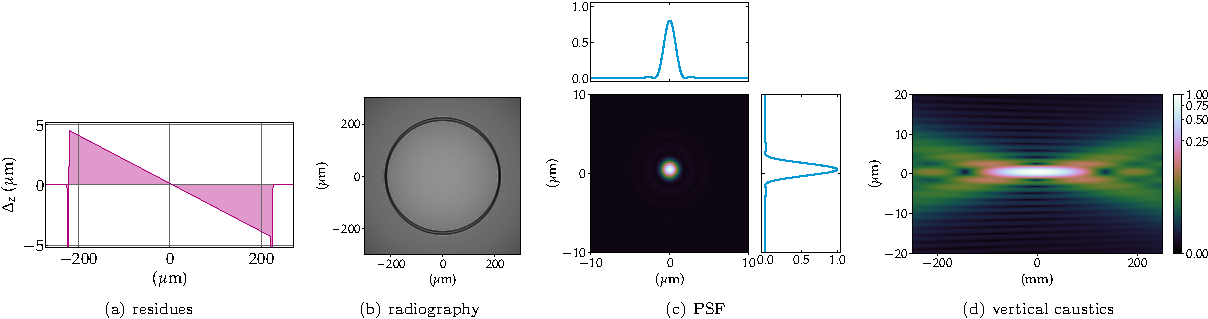
\includegraphics[height=4.19cm]{figures/ch04/offset_fs_CRL.pdf}
        \caption[Effects of the transverse offset of the parabolic section]{Simulations of a lens with front focusing parabolic section shifted by $\Delta_y=-2~\mu$m and back focusing shifted by $\Delta_y=-3~\mu$m - cf. Fig~\ref{fig:lens_cuts}(e). (a) Residual thickness, (b) phase-contrast image $150~$mm downstream the lens, (c) point spread function with cuts centred in $(0,0)$ and (c) the vertical beam caustics from $-250$~mm to $250$~mm in respect to the focal plane at $f=4.700~$m.} \label{fig:offset_fs_CRL}
\end{figure}

%-------------------------------------------------------------------------
%-------------------------------------------------------------------------
\subsubsection*{Tilted parabolic section}
%-------------------------------------------------------------------------
%-------------------------------------------------------------------------

When the axes of the parabolic front or/and back surfaces are not parallel to the optical axis, the lens active area appears to be tilted as shown in Figs.~\ref{fig:lens_cuts}(f)~and~(g). Similarly to what was introduced in the section \textit{Tilted lens} from \S\ref{sec:misalignments}~-~\textit{\nameref{sec:misalignments}}, both front and back surfaces are rotated according to the rotation matrices described in Eqs.~\ref{eq:affine} and the procedure described by Eq.~\ref{eq:affine2}. There are two subtle differences: the rotation angles from front and back surfaces can be chosen independently and rotation is only applied to the lens geometric aperture, and not to the whole front and back surfaces. The independent rotations allow for different regimes: one where both imprints are tilted with the same angle as in shown in Fig.~\ref{fig:lens_cuts}(f), which yields a residual phase similar to the one discussed in \textit{Tilted lens} from \S\ref{sec:misalignments}~-~\textit{\nameref{sec:misalignments}} and  one where there is no match of the front and back surfaces tilt, which yields an asymmetric residual phase as shown in Fig.~\ref{fig:tilt_fs_CRL}. By not applying the rotation to the region outside the lens geometric aperture, one avoids changing the lens projected thickness.

\begin{figure}[t]
        \centering
        {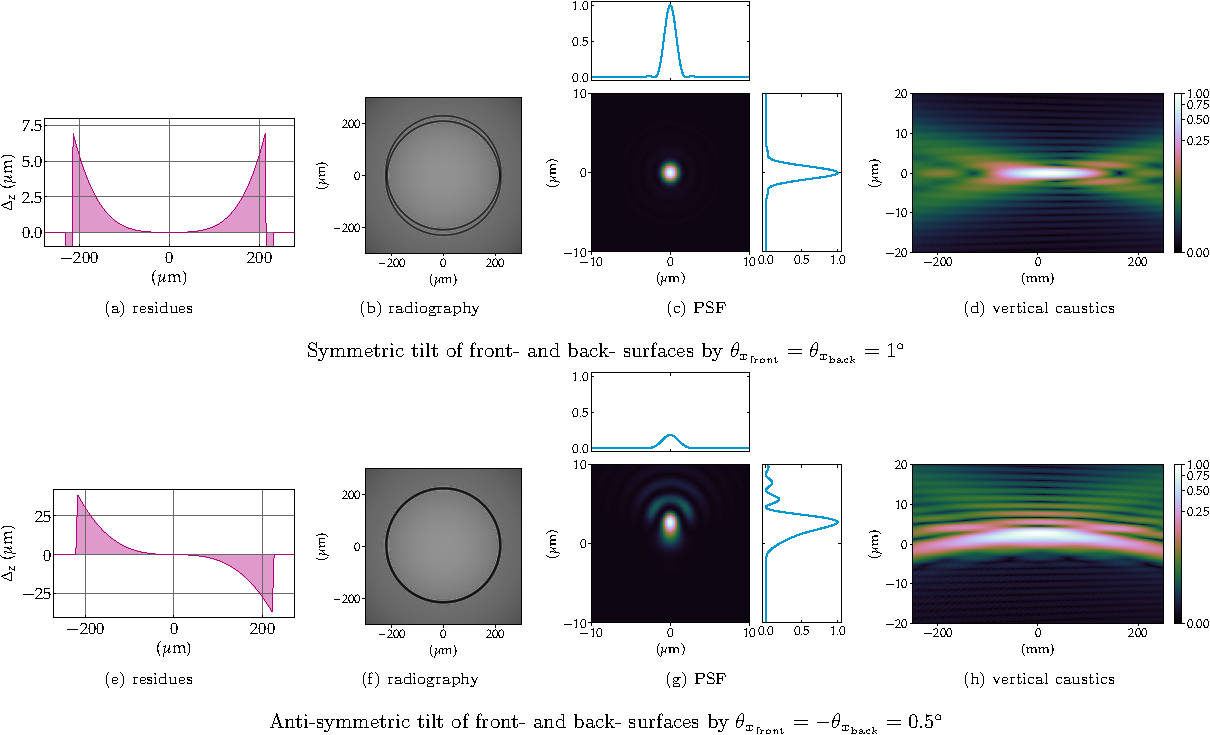
\includegraphics[width=1.\linewidth]{figures/ch04/tilt_fs_CRL.pdf}}
        \caption[Effects of the tilted parabolic section]{Simulations of a lens with front and back focusing parabolic sections independently tilted and shown in Fig~\ref{fig:lens_cuts}(f) and (g). The (a) residual thickness, (b) phase-contrast image $150~$mm downstream the lens, (c) point spread function with cuts centred in $(0,0)$ and (c) the vertical beam caustics from $-250$~mm to $250$~mm in respect to the focal plane at $f=4.700~$m of the symmetric tilt are shown on the top row. The (e) residual thickness, (f) phase-contrast image, (g) point spread function and (h) the vertical beam caustics for the anty-symmetric case with the same conditions is presented in the bottom row. While the symmetric case has a residual phase proportional to the 4$^{\text{th}}$ power of the lateral coordinates in the direction of the tilt, elongating the beam focusing in the propagation direction and shifting it on the same direction - typical of spherical aberrations, the residual phase of the anti-symmetric case has residual phase proportional to the 3$^{\text{rd}}$ power of the lateral coordinates in the direction of the tilt and has a PSF typical of coma-aberrated systems.  } \label{fig:tilt_fs_CRL}
\end{figure}

%-------------------------------------------------------------------------
%-------------------------------------------------------------------------
\subsection{Other sources of deviations from the parabolic shape}
%-------------------------------------------------------------------------
%-------------------------------------------------------------------------

So far, the modelling described here relies on translations and rotations of an ideal parabolic surface and investigating the residual phase. Another equally valid approach is to manipulate directly the residual phase and add it to the phase of an ideal focusing lens, which can be done fitting arbitrary surfaces or by introducing data from metrology of the optical element to be simulated.

\begin{figure}[t]
        \centering
        {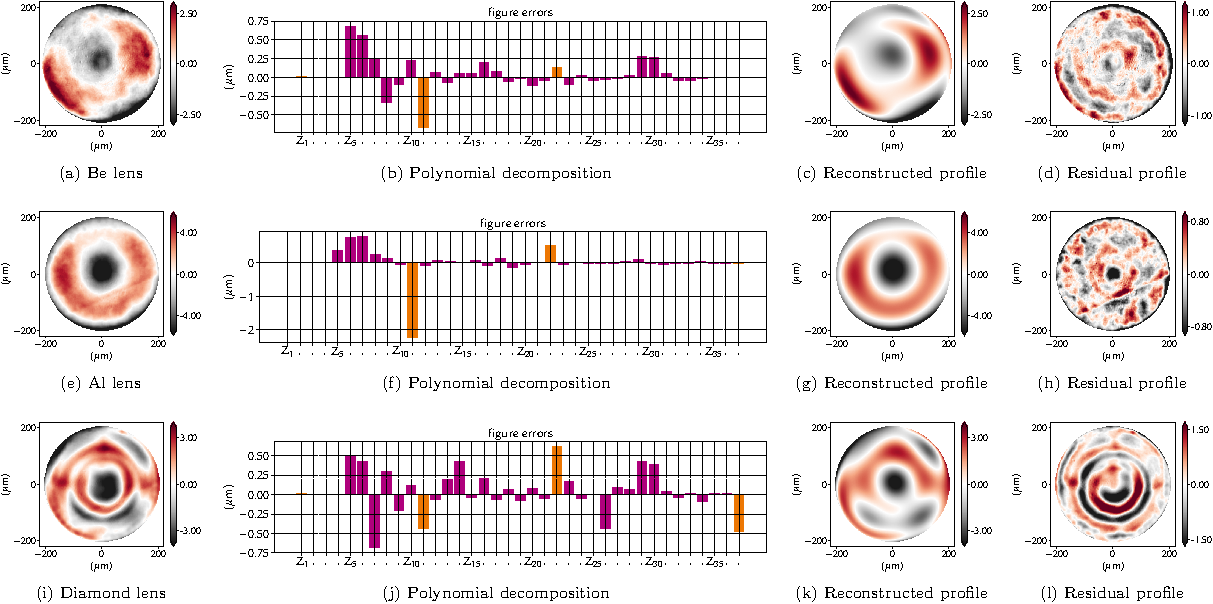
\includegraphics[width=1.\linewidth]{figures/ch04/metrology_zernike_profiles.pdf}}
        \caption[Other sources of deviations from the parabolic shape]{\textbf{First row}: (a) accumulated profile with RMS value: $\sigma_z=1.4~\mu$m, (b) Zernike circle polynomial decomposition of the profile in (a) and (c) the reconstruction based on the coefficients of a 2D-Beryllium lens with nominal radius $R\sim47.3~\mu\text{m}$ and useful aperture $A_{\diameter}\sim417~\mu\text{m}$ with RMS value: $\sigma_z=1.3~\mu$m. \textbf{Middle row}: (d) accumulated profile with RMS value: $\sigma_z=2.6~\mu$m, (e) Zernike circle polynomial decomposition of the profile in (d) and (f) the reconstruction based on the coefficients of a 2D-Aluminium lens with nominal radius $R\sim46.2~\mu\text{m}$ and useful aperture $A_{\diameter}\sim396~\mu\text{m}$ with RMS value: $\sigma_z=2.5~\mu$m. \textbf{Bottom row}: (g) accumulated profile with RMS value: $\sigma_z=1.8~\mu$m, (f) Zernike circle polynomial decomposition of the profile in (g) and (h) the reconstruction based on the coefficients of a 2D-diamond lens with nominal radius $R\sim103.4~\mu\text{m}$ and useful aperture $A_{\diameter}\sim402~\mu\text{m}$ with RMS value: $\sigma_z=1.6~\mu$m.}
        \label{fig:metrology_zernike_profiles}
\end{figure}

\begin{figure}[t]
        \centering
        {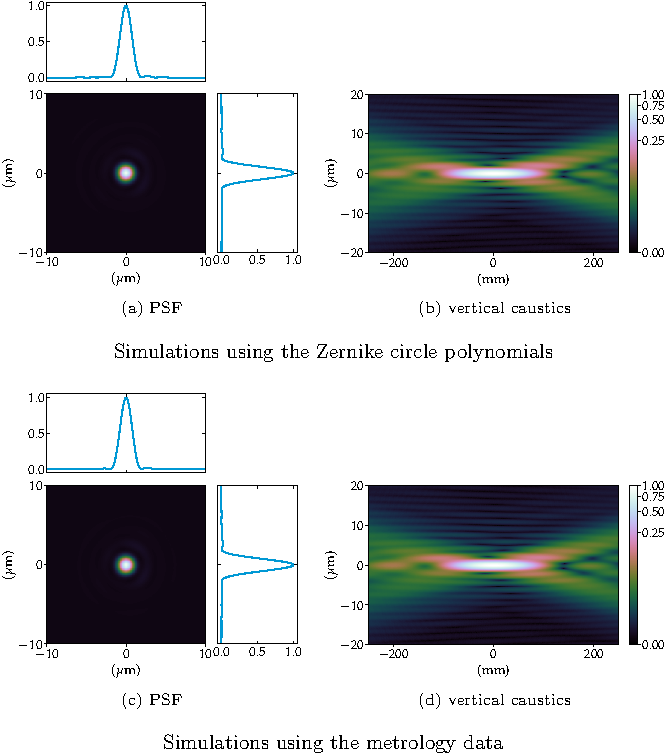
\includegraphics[height=11cm]{figures/ch04/metrology_zernike_simualtions.pdf}}
        \caption[Effects of other sources of deviations from the parabolic shape]{Simulations of a single 2D-Beryllium lens with nominal radius $R=50~\mu\text{m}$, geometric aperture $A_{\diameter}=440~\mu\text{m}$ and $t_\text{wall}=20~\mu$m at 8~keV. (a) and (c) point-spread function with cuts centred in $(0,0)$. (b) and (d) vertical beam caustics from -250~mm to 250~mm in respect to the focal plane. The difference between both profiles is almost not perceivable. This can be explained by the fact that the difference between the figure errors RMS value is almost negligible:  $\sigma_z=1.3~\mu$m (Zernike polynomial reconstruction) against $\sigma_z=1.4~\mu$m (metrology data), while the Mar\'echal criterion calculated for Beryllium lenses illuminated at $8$~keV requires the accumulated projected figure errors to be $\sigma_z\leq2.08~\mu$m, which makes the impact in the the reduction in intensity at the focal position is almost negligible - cf. Eqs.~\ref{eq:Strehl}-\ref{eq:ThickLim} for the Mar\'echal criteria and Strehl ratio in \textit{CRL performance: tolerance conditions for aberrations} from \S\ref{sec:refractive_optics}~-~\textit{\nameref{sec:refractive_optics}}.}\label{fig:metrology_zernike_simualtions}
\end{figure}

%-------------------------------------------------------------------------
%-------------------------------------------------------------------------
\subsubsection*{Orthornormal polynomials}
%-------------------------------------------------------------------------
%-------------------------------------------------------------------------

A widespread form of representing optical aberrations of arbitrary shapes is by decomposing them into an orthonormal base. Perhaps the most ubiquitous set of aberration functions is given by the Zernike polynomials for a circular aperture, first described in [\cite{Zernike1934}]. Their appeal comes from the fact that not only they are directly related to Seidel (primary), Schwarzschild (secondary) and tertiary-aberrations\footnote{This jargon comes from a power-series expansion of the aberration function. There are five primary aberrations, nine secondary aberrations and fourteen aberration terms for the tertiary aberrations. They all involve spherical aberration, coma, astigmatism, field
curvature, distortion and variations of thereof [\cite{Mahajan2013}].} but also include piston and tilts; they form an orthonormal base, which means that the value of the coefficients is not affected by the removal of a particular term [\cite{Mahajan2007}]. Another advantage of the Zernike polynomial decomposition is that each orthonormal aberration coefficient is the standard deviation for that particular aberration over the exit pupil, which is valuable when evaluating the optical system compliance with the  Mar\'echal criteria and calculating the Strehl ratio [\cite{Mahajan1983}].

For the aforementioned decomposition of the aberration function in an orthonormal base to retain its properties, the application of the circular Zernike polynomials must be limited to circular apertures. Other shapes of apertures with- or without obscuration can be obtained by Gram-Schmidt orthonormalisation and weighting of the Zernike circle polynomials [\cite{Swantner1994,Mahajan1995}]. X-ray optics systems often have a rectangular aperture and other two sets of polynomials are of particular interest in optical design: the set of orthonormal Zernike polynomials for a rectangular aperture  [\cite{Mahajan2007}] and the 2D-Legendre polynomial set for a rectangular aperture [\cite{Mahajan2010}]. Preferentially\footnote{Acknowledgments to Prof. V. Mahajan (University of Arizona, USA) and Prof. H. Gross (University of Jena, Germany) for the discussions on orthonormal polynomials in wavefront analysis and pointing out relevant literature.}, the Zernike circle polynomials are applied to 2D focusing lenses with a circular aperture. For 2D focusing X-ray lenses with square aperture, low aspect ratio between horizontal and vertical apertures and not strongly astigmatic focusing, e.g. crossed planar X-ray lenses, the Zernike rectangular polynomials are preferred. The 1D focusing lens is better fit by the 2D Legendre polynomial set\footnote{Please, refer to [\cite{Ye2014}] for a comparison between 2D orthonormal sets for square apertures.}. Analysing and describing refractive X-ray optics using circular Zernike and 2D Legendre polynomials were first presented by [\cite{Koch2016}]. Profiles generated by Zernike circle polynomials are shown in the right-hand side of Fig.~\ref{fig:metrology_zernike_profiles} and their effect on a coherent X-ray beam in Fig.~\ref{fig:metrology_zernike_simualtions}(a) and (b).

\newpage
%-------------------------------------------------------------------------
%-------------------------------------------------------------------------
\subsubsection*{Metrology data}
%-------------------------------------------------------------------------
%-------------------------------------------------------------------------

Any (unintentional) deviation of a parabolic shape can be considered as a source of manufacturing error. Each manufacturing process has some type of (signature) error associated to it and with the increasing number of exotic - or non-conventional - designs and tailored manufacturing strategies, it is beyond reasonable to create a model that could parametrise all sources of deviations from the parabolic shape. To circumvent that and to accurately model phase imperfection in compound refractive lenses, metrology data can also be used for optically imperfect X-ray lenses [\cite{Celestre2020, Chubar2020}]. Fig.~\ref{fig:metrology_zernike_profiles} shows three examples of lens figure errors from (a)-(c) a commercial pressed Beryllium lens, (d)-(f) an in-house pressed Aluminium lens and a (g)-(h) in-development laser-ablated Diamond lens from a commercial partner. The figure errors were measured with at-wavelength metrology\footnote{cf. \S\ref{sec:at_wavelength}~-~\textit{\nameref{sec:at_wavelength}}.} and can be directly plugged into simulations [\cite{Celestre2020}]. The effect on a coherent X-ray of optical imperfections from metrology data is shown in Fig.~\ref{fig:metrology_zernike_simualtions}(c) and (d).

\begin{figure}[t]
        \centering
        {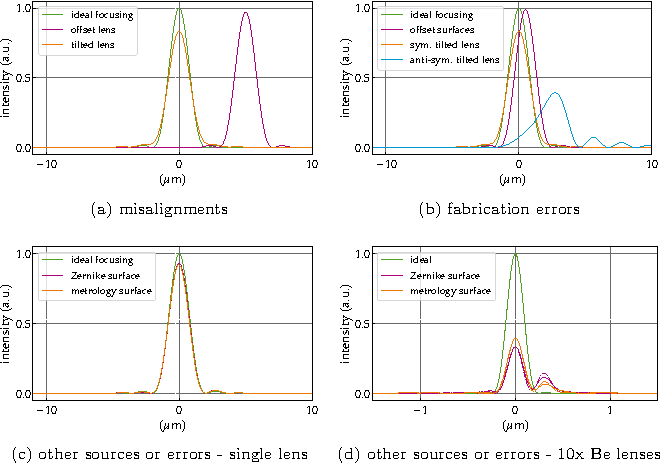
\includegraphics[width=1.\linewidth]{figures/ch04/Strehl}}
        \caption[Strehl ratio summarising the results from the diverse models presented]{Strehl ratio of the vertical cut at $x=0$ summarising the results from the diverse models presented.} \label{fig:Strehl_modelling}
\end{figure}

%-------------------------------------------------------------------------
%-------------------------------------------------------------------------
\subsection{Implementation}
%-------------------------------------------------------------------------
%-------------------------------------------------------------------------

The implementation of the modelling of the CRL, its misalignments and its figure errors is done using Python 3.7 and is fully compatible with the optical element class \texttt{SRWLOpt} described in the module \texttt{srwlib.py} from SRW\footnote{\url{github.com/ochubar/SRW}}. Each function representing either an X-ray lens or its figure errors returns a class \texttt{SRWLOptT} representing a generic transmission element storing amplitude transmission and optical path difference as a function of transverse coordinates. The main calculations for generating the X-ray lens transmission element is performed by the function \texttt{srwl\_opt\_setup\_CRL}. Apart from generating an ideal CRL (cf. Eq.~\ref{eq:TE_singlelens}), this function implements the degrees of freedom discussed in \S\ref{sec:misalignments}~-~\textit{\nameref{sec:misalignments}}; longitudinal and transverse offsets as well as the tilts of the individual parabolic sections as described in \S\ref{sec:fabrication}~-~\textit{\nameref{sec:fabrication}}. The generation of the residual phase errors based on the polynomial expansion of the aberration function in the exit pupil is done by \texttt{srwl\_opt\_setup\_CRL\_errors}. To calculate the aberration function, the user can either use a list with the polynomial coefficients or enter an RMS value for their sum (equivalent to fixing the piston value), in which case, they will be randomly calculated will comply with the RMS value limited by the user input. This function generates the residual errors and should be used in conjunction with \texttt{srwl\_opt\_setup\_CRL} to simulate an aberrated focusing lens. The aberration functions in \texttt{srwl\_opt\_setup\_CRL\_errors}\footnote{The functions used by \texttt{srwl\_opt\_setup\_CRL\_errors} to generate the 2D circular Zernike polynomials contain pieces of codes from the module \texttt{libtim-py} from Tim van Werkhoven, that had to be brought to Python 3.7 and in some places, small bugs fixed - this module has a Creative Commons Attribution-Share Alike
license. The 2D rectangular Zernike was originally inspired by the analytical formulation from the module \texttt{opticspy} from Xing Fan - this module has an MIT license. The formulation from the module was based on the equations from [\cite{Mahajan2007}], but had to be corrected with the errata published in [\cite{Mahajan2012}].} use the analytical solutions from [\cite{Mahajan2007}] with the corrections from [\cite{Mahajan2012}] and the solutions from [\cite{Mahajan2010}].  The generation of a surface based on the metrology data is done by \texttt{srwl\_opt\_setup\_CRL\_metrology}. The metrology data should be saved as an ASCII file (.dat) as defined by the function \texttt{srwl\_uti\_save\_intens\_ascii} from the module \texttt{srwlib.py}. The function \texttt{srwl\_opt\_setup\_CRL\_metrology} can be used to simulate figure errors, in which case, much like \texttt{srwl\_opt\_setup\_CRL\_errors} it requires the use of \texttt{srwl\_opt\_setup\_CRL} or it can be used to simulate a full measured profile. This library extension is currently available under a CC BY-SA 4.0 license at the \href{https://gitlab.esrf.fr/celestre/barc4RefractiveOptics}{barc4RefractiveOptics} GitLab repository\footnote{\url{gitlab.esrf.fr/celestre/barc4RefractiveOptics}}, where more information on the implemented functions can be found.

%-------------------------------------------------------------------------
%-------------------------------------------------------------------------
\section{Measuring optical imperfections in refractive lenses}\label{sec:metrology}
%-------------------------------------------------------------------------
%-------------------------------------------------------------------------

Surface metrology methods commonly applied to X-ray mirrors [\cite{Alcock2016, Vivo2019}] are not broadly employed for the metrology of X-ray lenses mainly due to their small apertures and steep parabolic surfaces (cf. Fig.~\ref{fig:ideal_CRL}) [\cite{Lyatun2015}]. Non-destructive methods using X-rays are often more appropriate for X-ray lens metrology. This section presents some of the commonly used at-wavelength metrology methods, with emphasis on X-ray speckle vectorial tracking, the experimental technique used throughout this work. The metrology of single- and stacked 2D-Beryllium lens with $R=50~\mu$m is presented and the results are compared. A framework for calculating corrective optics for such stacked lenses is shown, along with the first correction prototypes and tests.

The experimental data shown in this section was taken on several beamtimes\footnote{Acknowledgements to Sébastien Bérujon and Ruxandra Cojocaru (BM05-ESRF); Xianbo Shi, Zhi Qiao, Michael Wojcik and Lahsen Assoufid (1-BM-APS); and to Carsten Detlefs (ID06-ESRF) for the help during the experimental sessions.} at the BM05 beamline - ESRF [\cite{Ziegler2004}] (from 2017 to 2018 - before the ESRF long shutdown for the EBS upgrade), at the 1-BM beamline - APS [\cite{Macrander2016}] (in 2019 during the ESRF long shutdown) and the ID06 beamline - ESRF [\cite{Kutsal_2019}] (in 2020 in the commissioning period of the ESRF-EBS upgrade).


%-------------------------------------------------------------------------
%-------------------------------------------------------------------------
\subsection{At wavelength-metrology}\label{sec:at_wavelength}
%-------------------------------------------------------------------------
%-------------------------------------------------------------------------

Surface metrology of X-ray optical elements is often done using visible spectral range [\cite{Alcock2016, Vivo2019}] even if, ultimately, they will be employed in a total different spectral range. At-wavelength metrology is an umbrella term for measurements of optical elements at wavelengths closer to the ones they will be ultimately used - in the case of X-ray lenses, a few dozen kilo-electron-volts. What follows is a non-exhaustive description of commonly used techniques for quality control applied to X-ray lenses and their compliance to a parabolic shape. Other relevant at-wavelength characterisation of X-ray lenses such as X-ray small angle scattering [\cite{Roth2014, Chubar2020}] or the impact of material micro-structures or shape errors on imaging [\cite{Chubar2020,Lyatun2020}] are not covered. 

The simplest techniques involve direct imaging the lens with X-rays by propagation-based phase contrast imaging [\cite{Endrizzi2018}], since absorption contrast imaging has a very reduced contrast for a single lens. With such simple techniques, 2D shapes and distances can be measured (radiographs for controlling the distance and alignment between the parabolic surfaces of X-ray lenses). Still based on imaging techniques, X-ray laminography [\cite{Helfen2011,Roth2014}] and X-ray tomography [\cite{Landis2010,Narikovich2017}] of X-ray lenses provide a 3D reconstruction of the lens volume with high spatial resolution information. These techniques provide data on the refracting surfaces shape and on the internal features (inhomogeneities) and can be used for modelling optical imperfections in refractive lenses. 


Another large family of experimental techniques used for lens metrology can be grouped under the wave-front sensing branch\footnote{With the advent of more coherent sources of X-rays as encapsulated by the emmergence of $4^{\text{th}}$-generation synchrotrons and free-electron lasers, the topic of wavefront sensing has seen increased attention [\cite{Seaberg2019}].}. Wavefront-sensing is often employed as a beam-diagnostics tool for highly coherent sources [\cite{Seaberg2019}]. Two approaches are often used: \textit{i}-) the absolute wavefront after an specific optical element is measured and the global state of the wavefront is obtained or \textit{ii}-) a differential measurement is done with and without the optical element under investigation, the differences in the wavefront attributed to the addition of the optical element under test. Current wavefront-sensing techniques used for evaluating the phase errors of CRLs (or individual X-ray lenses) are: the Ronchi test, an interferometric technique that provides qualitative\footnote{It has been demonstrated that the Ronchi test can also retrieve quantitative information [\cite{Lee2010}], but is has not yet been applied to X-ray lenses metrology.} information on third order optical aberrations [\cite{Nilsson2012, Uhlen2014}]; the use of X-ray Shack–Hartmann sensors [\cite{Mayo2004,Mikhaylov2020}]; the ptychographic reconstruction of the wavefront emerging from a strong focusing optics [\cite{Schropp2013,Sala2017,Seiboth2017}]; grating interferometry and all its variations [\cite{David2012,Koch2016,Grizolli2017}]; and the near-field-speckle-tracking-based methods [\cite{Berujon2013,Zdora2018,Berujon2020a}].

%-------------------------------------------------------------------------
%-------------------------------------------------------------------------
\subsubsection*{X-ray (near field) speckle vector tracking (XSVT)}\addcontentsline{toc}{subsubsection}{-- X-ray (near field) speckle vector tracking (XSVT)}
%-------------------------------------------------------------------------
%-------------------------------------------------------------------------

The X-ray near-field-speckle-tracking is the chosen technique for systematic at-wavelength metrology of X-ray lenses at the ESRF\footnote{Other synchrotron facilities also offer X-ray lens metrology with the X-ray near field speckle tracking technique: 1-BM at the APS in the U.S.A. [\cite{Qiao2020}] and the B16 beamline at the Diamond Light Source in the U.K. [\cite{Sawhney2013}].} and is available at the BM05 beamline [\cite{Berujon2020a}] and most recently, at the ID06 beamline. The principal reasons for this choice are: \textit{i}-) the lower requirements on transverse- and longitudinal coherence [\cite{Zanette2014,Zdora2015}]; \textit{ii}-) no requirement of specially tailored optics (nor accompanying complicated alignment procedures) [\cite{Morgan2012,Wang2016}]; \textit{iii}-) successful benchmark against more established wave-front sensing techniques [\cite{Kashyap2016,Romell2017}]; and \textit{iv}-) its versatility as a metrology tool being able to measure mirrors, single- and stacked lenses [\cite{Berujon2020a}]. Although the basic principles of the the several X-ray near-field-speckle-based techniques are the same, focus is given to the X-ray (near field) speckle vector tracking (XSVT) as implemented and used for the metrology of single- and stacked X-ray lenses used in this work [\cite{Berujon2020a,Berujon2020}]. An interesting review on different techniques using X-ray near field speckle tracking is given by [\cite{Zdora2018a}] and [\cite{Berujon2020}].

%-------------------------------------------------------------------------
%-------------------------------------------------------------------------
\subsubsection*{-- Introduction}
%-------------------------------------------------------------------------
%-------------------------------------------------------------------------

\begin{figure}[t]
        \centering
        {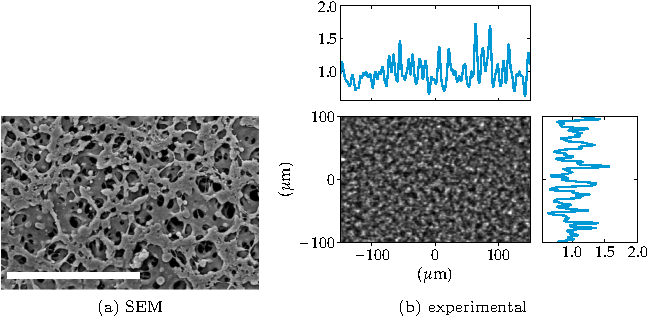
\includegraphics[width=0.6\linewidth]{figures/ch04/SpecklePattern.pdf}}
        \caption[Speckle-pattern and the stationary diffuser]{(a) Speckle-pattern measured at 17~keV at 800~mm downstream the with $\sigma_I=0.19$~a.u., $\overline{I}=0.99$~a.u. and $v\sim0.19$; (b) SEM image of the cellulose acetate membrane filters with mean pore size of 1.2~$\mu$m used as the stationary diffuser. The white bar represents 50~$\mu$m.} \label{fig:SpecklePattern}
\end{figure}


Near-field speckle is a manifestation in intensity of the summation of several complex electric fields when the amplitudes and phases of such fields have random values. The resulting intensities may be locally high due to constructive interference or low, due to destructive interference [\cite[\textit{\S1}]{Goodman2020}]. Globally, to a speckle pattern over a defined region of interest, the speckle contrast (or visibility) can be defined\footnote{Other definitions are commonly found in the literature: $v=\frac{I_\text{max}-I_\text{min}}{I_\text{max}-I_\text{min}}$ and $v=\frac{I_\text{max}-I_\text{min}}{2\overline{I}}$, where $I_\text{max}$ and $I_\text{min}$ are the maximum and minimum intensities found in the region of interest [\cite{Zdora2018a}].} as:
\begin{equation}\label{eq:visibility}
    v=\frac{\sigma_I}{\overline{I}},
\end{equation}
where $\sigma_I$ is the standard deviation and $\overline{I}$ is the mean value of the intensity value of the speckle pattern. In the X-ray regime, it appears when a sufficiently coherent X-ray beam is transmitted through matter with random spatial variation of $\delta$ and $\beta$, where the local optical path length varies significant when compared to the scale of the wavelength.

For a static random modulation of the wavefield (stationary diffuser\footnote{As opposed to time-varying modulation of the speckle-field as in \cite{Morgan2010,Goikhman2015}.}), it has been demonstrated that the speckle-grains\footnote{Continous regions in space with slowly-varying intensity that can be visually clustered together.} preserve shape and size for free-space propagation distances limited to:
\begin{equation}\label{eq:speckle_goodness}
z<\Delta_{\textbf{cl}_\perp}\xi k,
\end{equation}
where $\Delta_{\textbf{cl}_\perp}$ is transverse coherence length\footnote{cf. \textit{Spatial coherence} in \S\ref{sec:optical_coherence}~-~\textit{\nameref{sec:optical_coherence}}.} and $\xi$ is the typical transverse length of the modulator, that is, the region where the spatial variation of $\delta$ and $\beta$ is negligible [\cite{Cerbino2008}]. For propagation distances smaller than the imposed limit in Eq.~\ref{eq:speckle_goodness}, speckles can be used as a wavefront marker, since the transverse position of the speckle grains in two parallel planes along the propagation direction can be inferred geometrically. The near-field regime is of particular interest for the X-ray energy range, as very low wavelengths lead to an extended near-field regime. A speckle-pattern and the stationary diffuser used to generate it are shown in Fig.~\ref{fig:SpecklePattern}.

\begin{figure}[t]
        \centering
        {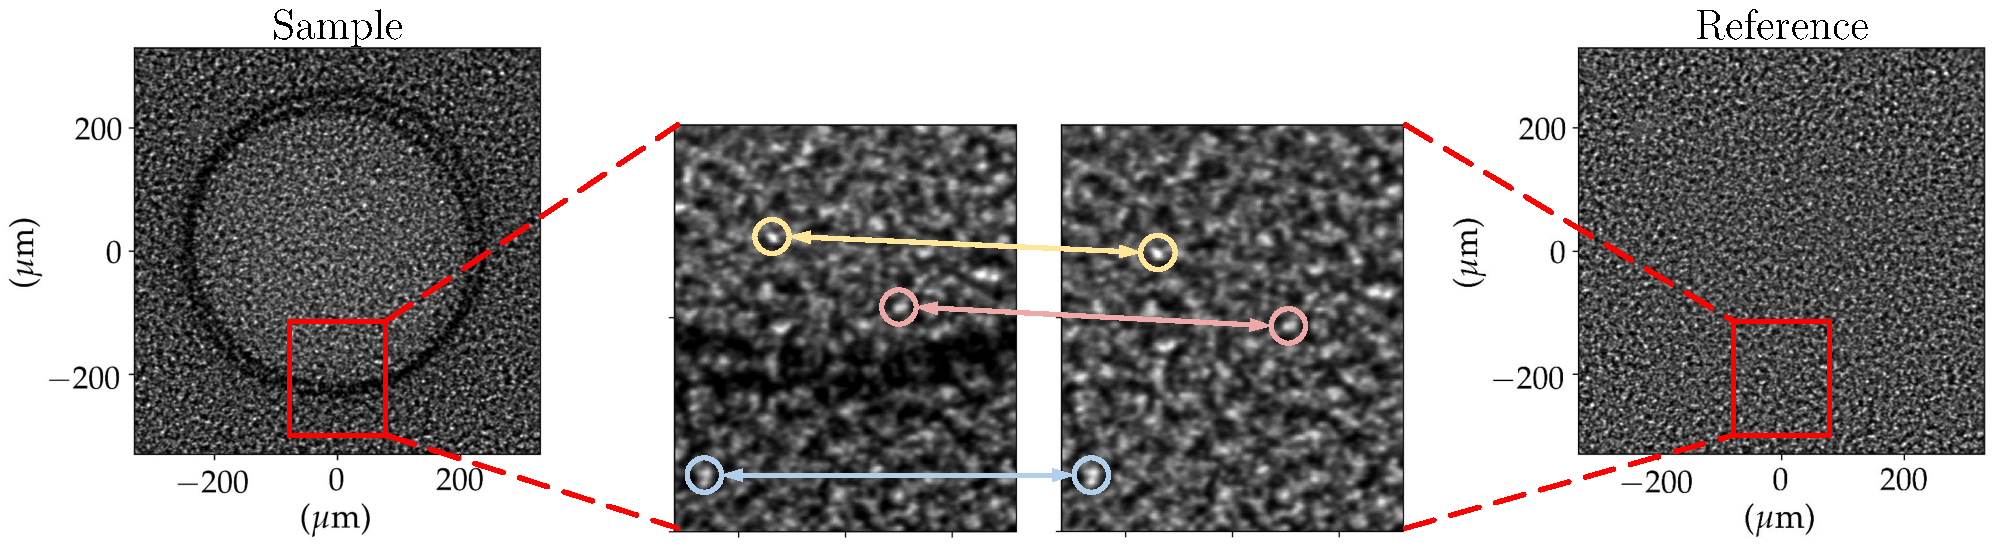
\includegraphics[width=1\linewidth]{figures/ch04/speckle_tracking.pdf}}
        \caption[Tracking of speckle grain]{Tracking of speckle grains. The highlighted grains in yellow and red are inside the sample and have their transverse position changed. The highlighted grain in blue is outside the lens active area and has no apparent shift in transverse position. The sample is a single 2D-Beryllium lens with nominal radius $R=50~\mu\text{m}$, geometric aperture $A_{\diameter}\sim440~\mu\text{m}$. The data was collected $\sim$800mm downstream the speckle-membrane at 17~keV.} \label{fig:speckle_tracking}
\end{figure}

\begin{figure}[t]
        \centering
        {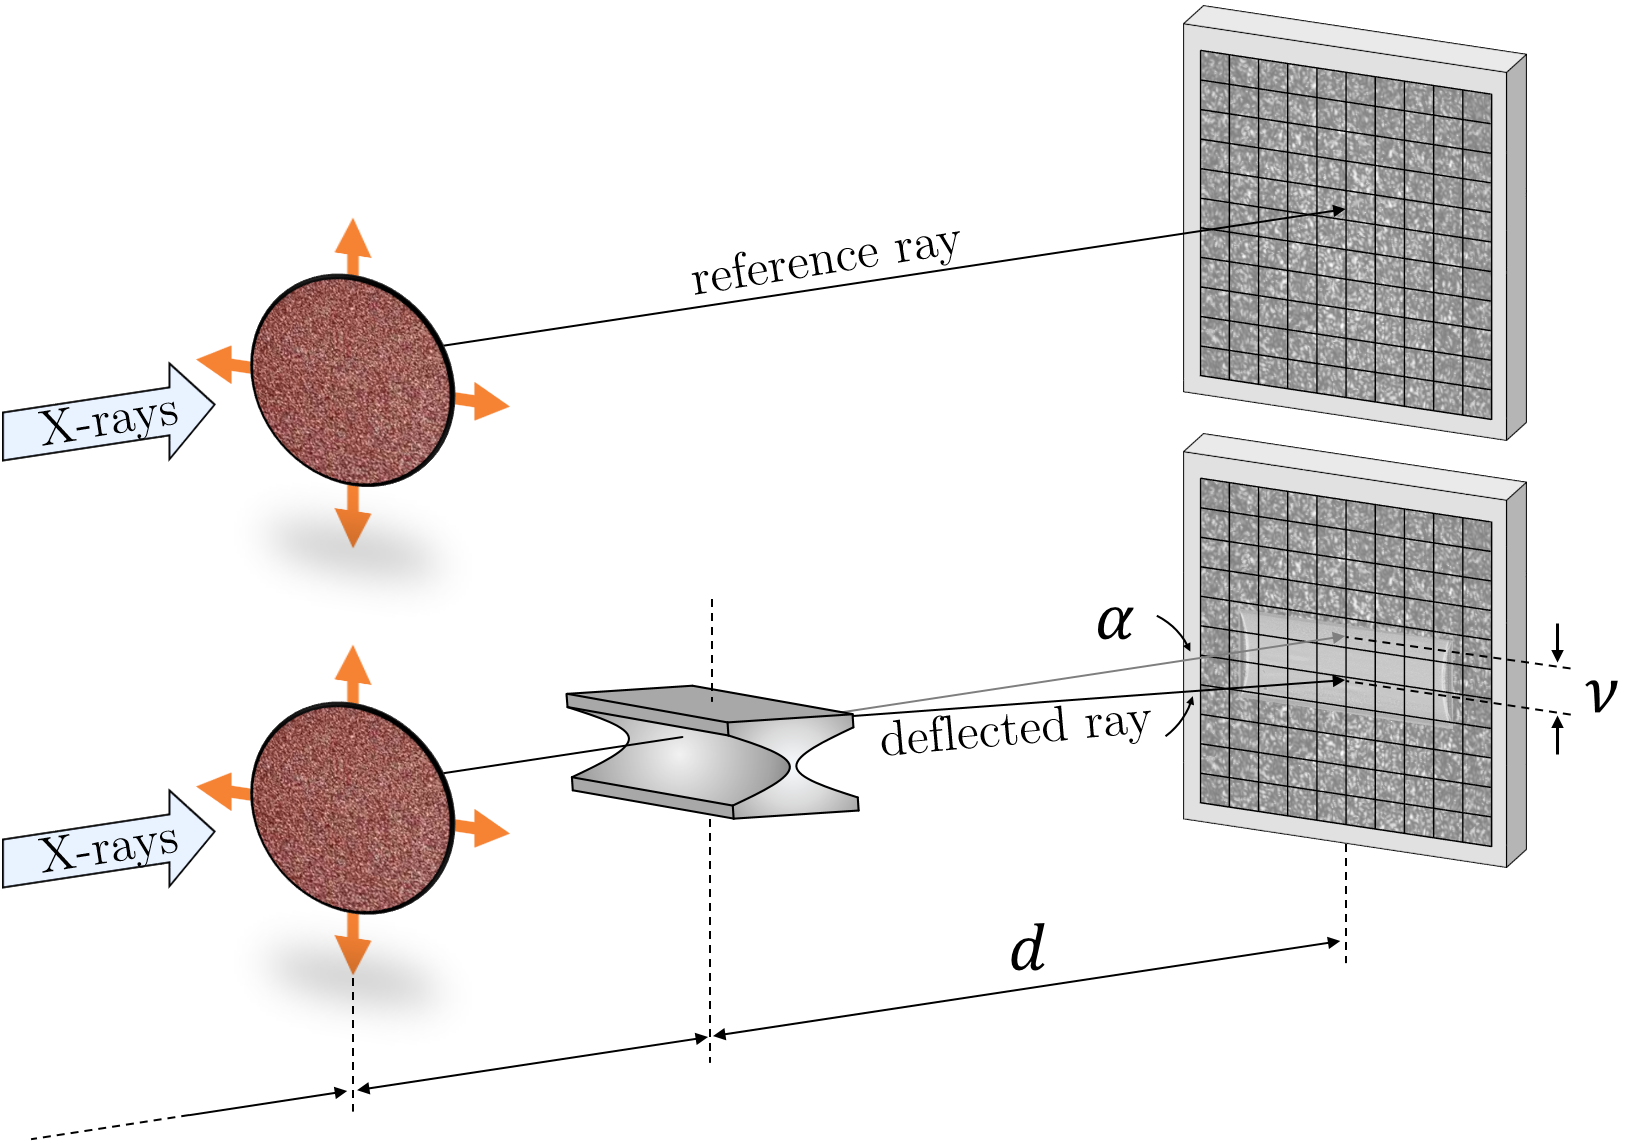
\includegraphics[width=0.6\linewidth]{figures/ch04/speckle_tracking2.png}}
        \caption[Speckle tracking geometry]{Generic speckle-tracking measurement geometry for the XSVT technique and the origin of the displacement vector $\nu$. From left to right: X-ray beam, speckle-membrane, sample and 2D imaging detector. The distance between sample and detector is given by $d$, the deflection angle is $\alpha$ and the transverse displacement vector in the detector plane is $\nu$.} \label{fig:speckle_tracking2}
\end{figure}

Based on the uniqueness of each speckle grain, speckle-tracking-based techniques rely on identifying similar patterns in two different images sets: reference image and in the presence of the probe (perturbed) - cf. Fig.~\ref{fig:speckle_tracking}. The computer implementations used for numerically tracking the lateral displacement of the speckle grains in the detector plane vary: cross-correlation peak calculation [\cite{Berujon2012, Morgan2012}] and the least-square-minimisation [\cite{Zanette2014, Zdora2017}] are the two most ubiquitous methods\footnote{Recently, a Euclidean-distance minimisation of the wavelet-transform method has been reported. Compared to correlation-based techniques it is less computationally demanding and more robust to noise [\cite{Qiao2020b}].}$^{,}$\footnote{Regardless of the tracking method, the displacement vector $\nu$ should be equivalent, as it is intimately linked to the sample shape and material.}. The lateral displacement of the speckle grain in the detector plane between the reference and the disturbed image is given by the displacement vector $\nu=(\Delta_x,\Delta_y)$, where $\Delta_x$ and $\Delta_y$ are the respective horizontal and vertical displacements of the speckle grain in the presence of the sample - cf. Fig.~\ref{fig:speckle_tracking2}. With knowledge of the distance between sample and detector $d$, it is possible to reconstruct the deflection angle $\alpha=(\alpha_x,\alpha_y)$ is given by $\alpha\approx\nu/d$. The deflection angle, the wave-field phase $\phi(x,y)$ and wavefront $\mathcal{W}(x,y)$ are related by:
\begin{equation}\label{eq:wavefront_gradient}
    k \alpha = \nabla\phi = k \nabla\mathcal{W}.
\end{equation}
The beam phase $\phi(x,y)$ or wavefront $\mathcal{W}(x,y)$ can be retrieved by numerical integration of the phase gradients obtained experimentally.

%-------------------------------------------------------------------------
%-------------------------------------------------------------------------
\subsubsection*{-- Experimental setup}
%-------------------------------------------------------------------------
%-------------------------------------------------------------------------

\begin{figure}[t]
        \centering
        {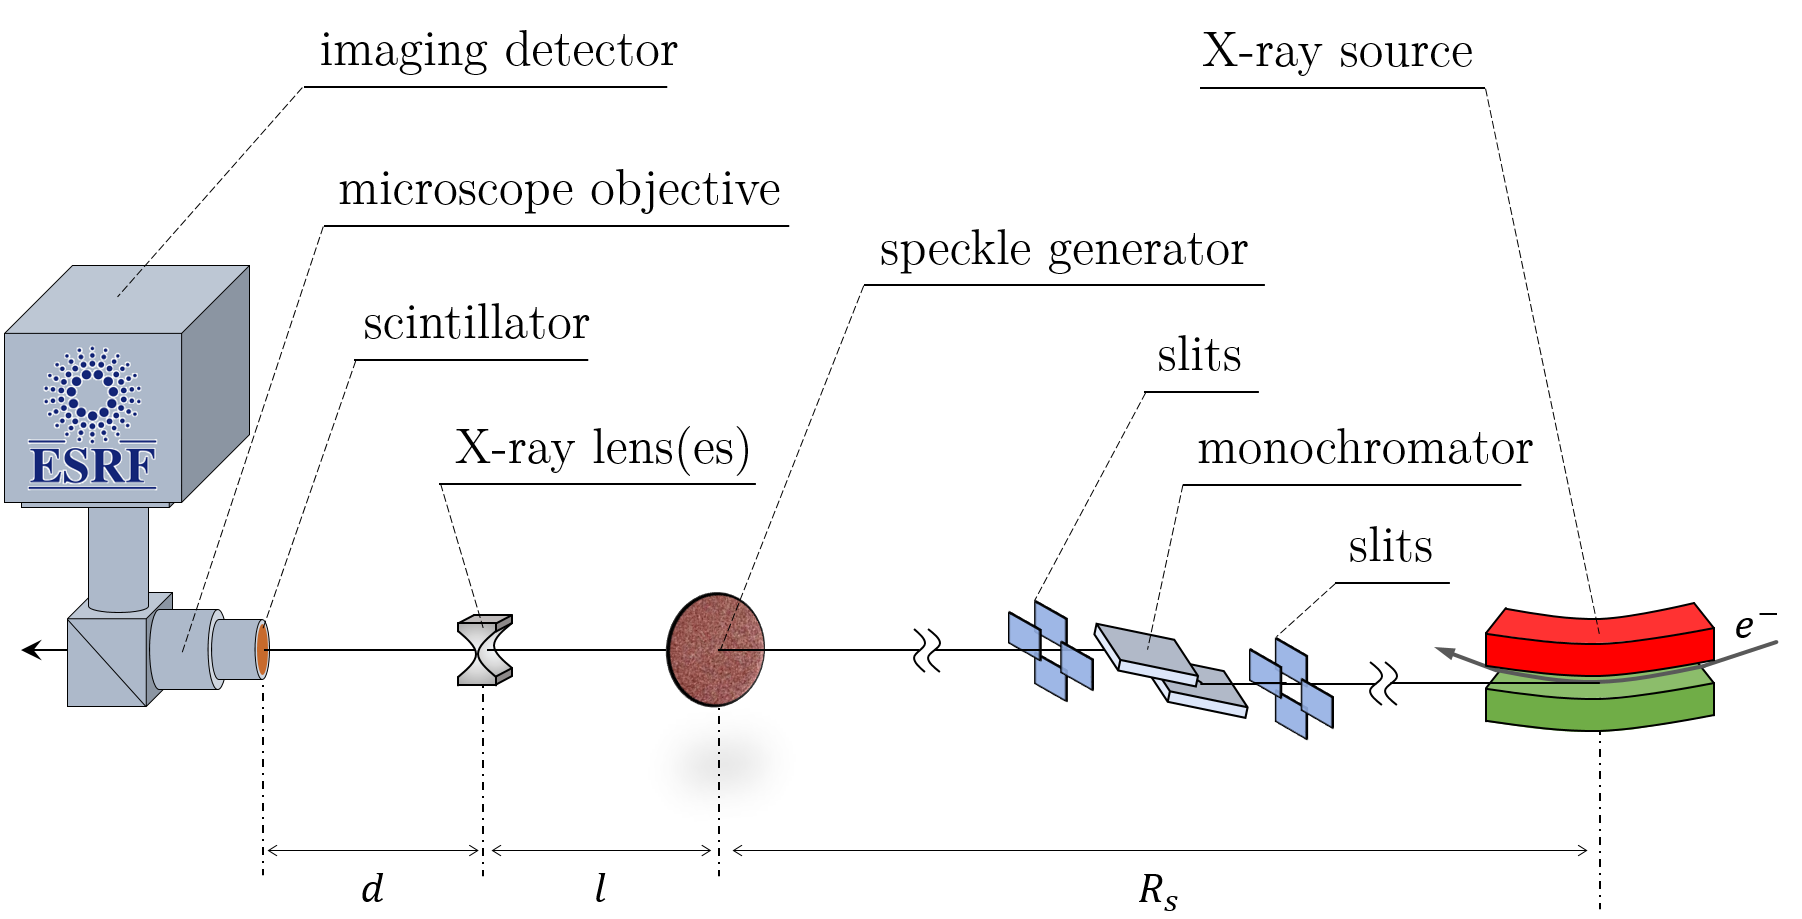
\includegraphics[width=0.7\linewidth]{figures/ch04/BM05.png}}
        \caption[Speckle tracking experimental setup at the BM05 beamline, ESRF.]{Generic speckle-tracking experimental setup as originally implemented in the BM05 beamline at the ESRF. \textbf{right to left}: an X-ray source (bending magnet) delivers a beam that has to be monochromatised by Si(111) double crystal monochromator down to a bandwidth of $\Delta \text{E}/\text{E}\approx10^{-4}$. The now monochromatised beam hits the speckle-generator at a distance $R_S$ from the source. The stationary diffuser is composed of several piled up cellulose acetate membrane filters with mean pore size of 1.2~$\mu$m. The membranes are mounted on a (piezoelectric) nano-positioner transverse translation stage, so that the membranes can be scanned on the $xy-$plane. At a distance $l$ downstream the membrane, the sample is placed and aligned as to the optical axis. Further downstream the probe, at a distance $d$, a 10~$\mu$m thick LSO:Tb scintillator converts the X-rays into visible light. The scintillator is imaged into a CMOS PCO Edge 4.2 or a FReLoN camera (2048 x 2048 pixels), which is coupled with a 10x magnification microscope objective in order to reach as theoretical pixel size of about $\sim0.62\times~0.62~\mu$m$^2$. Such experimental setup, without any structural change, was later on used at the 1-BM (APS) and ID06 (ESRF) beamlines. The X-ray source at the ID06 is an undulator and not a bending magnet as depicted here.} \label{fig:BM05}
\end{figure}

X-ray speckle-tracking can be implemented in several geometries depending on the metrology subject (mirrors, strong focusing mirrors, lenses, stacked lenses) and mode (absolute or differential) - cf. [\cite{Berujon2020a}]. In this section the X-ray (near field) speckle vector tracking (XSVT), a differential metrology mode, as originally implemented at BM05 and shown in Figs.~\ref{fig:speckle_tracking2} and \ref{fig:BM05} is described.




\footnote{At BM05, a bending magnet was the X-ray source until the ESRF-EBS upgrade. The long BM was decomissioned in favour of a much shorter and brighter 2-pole wiggler. All the data collected at BM05 was taken before this upgrade. At the 1-BM, the photon source is also a BM while at the ID06 the source is an undulator.}

 A highly coherent X-ray source will have a higher contrast when compared to a lower-coherence source for the same random modulation. The reduction in coherence leads to a smearing of the speckle pattern.
 
 This is done to ensure that the speckle-grain size covers a few pixels (<10 pixels). A minimum contrast of 0.1 (Eq.~\ref{eq:visibility}) is required, which is set by the transverse coherence length $\Delta_{\textbf{cl}_\perp}$ at the speckle generator position. At the cost of flux, the coherence length can be increase by slitting down the beam 
 at a good compromise between the visible light yield, resulting in lower integration times and lateral resolution.
[\cite{Berujon2020a, Berujon2020}]


%-------------------------------------------------------------------------
%-------------------------------------------------------------------------
\subsubsection*{-- Data acquisition, processing and analysis}
%-------------------------------------------------------------------------
%-------------------------------------------------------------------------


%-------------------------------------------------------------------------
%-------------------------------------------------------------------------
\subsection{Single lens measurements}
%-------------------------------------------------------------------------
%-------------------------------------------------------------------------

%-------------------------------------------------------------------------
%-------------------------------------------------------------------------
\subsection{Stacked lenses measurements}
%-------------------------------------------------------------------------
%-------------------------------------------------------------------------

%-------------------------------------------------------------------------
%-------------------------------------------------------------------------
\subsection{Corrective optics}
%-------------------------------------------------------------------------
%-------------------------------------------------------------------------

% %-------------------------------------------------------------------------

$\blacksquare$
\addcontentsline{toc}{section}{References}
\printbibliography[heading=subbibliography]
\end{refsection}

